\section{牛顿迭代法}
\subsection{牛顿迭代法的定义}
    牛顿迭代法(Newton's method)是牛顿在17世纪提出的一种在实数域和复数域上近似求解方程的方法。
    对于大多数方程而言求精确根非常困难,甚至存在不可解情况,
    从而求解这类方程的问题转为寻找方程的近似根。
    牛顿迭代法使用函数$f(x)$的泰勒级数的前面几项来寻找方程$f(x)=0$的根。
    假设目标函数$f(x)$在$x$处二阶可微,且当前的迭代点为$x_k$,
    那么在出的泰勒展开时为
    \begin{equation}
        f(x_k+d) = f_k + g_k^Td+\frac{1}{2}d^TG_kd + (\|d\|_2^2).
        \label{ndddf1}
    \end{equation}
    由于$d = x - x_k$,则式\ref{ndddf1}可转为式\ref{ndddf2}表达
    \begin{equation}
        \mathop{\mathrm{min}} q_k(d) = f_k + g_k^Td+\frac{1}{2}d^TG_kd.
        \label{ndddf2}
    \end{equation}
    若$G_k$正定,则方程组$G_kd=-g_k$的$d_k=-G_k^{-1}g_k$解为以上问题的唯一解。
    我们称上述方程组为牛顿方程组,
    解得的方向$d_k$为牛顿方向。
    用牛顿方向作为迭代方向的最优化方法称为牛顿方法。
    特别的,全步长$\alpha_k=1$的牛顿方法称为基本牛顿方法。
    \begin{figure}[hbtp]
        \centering
        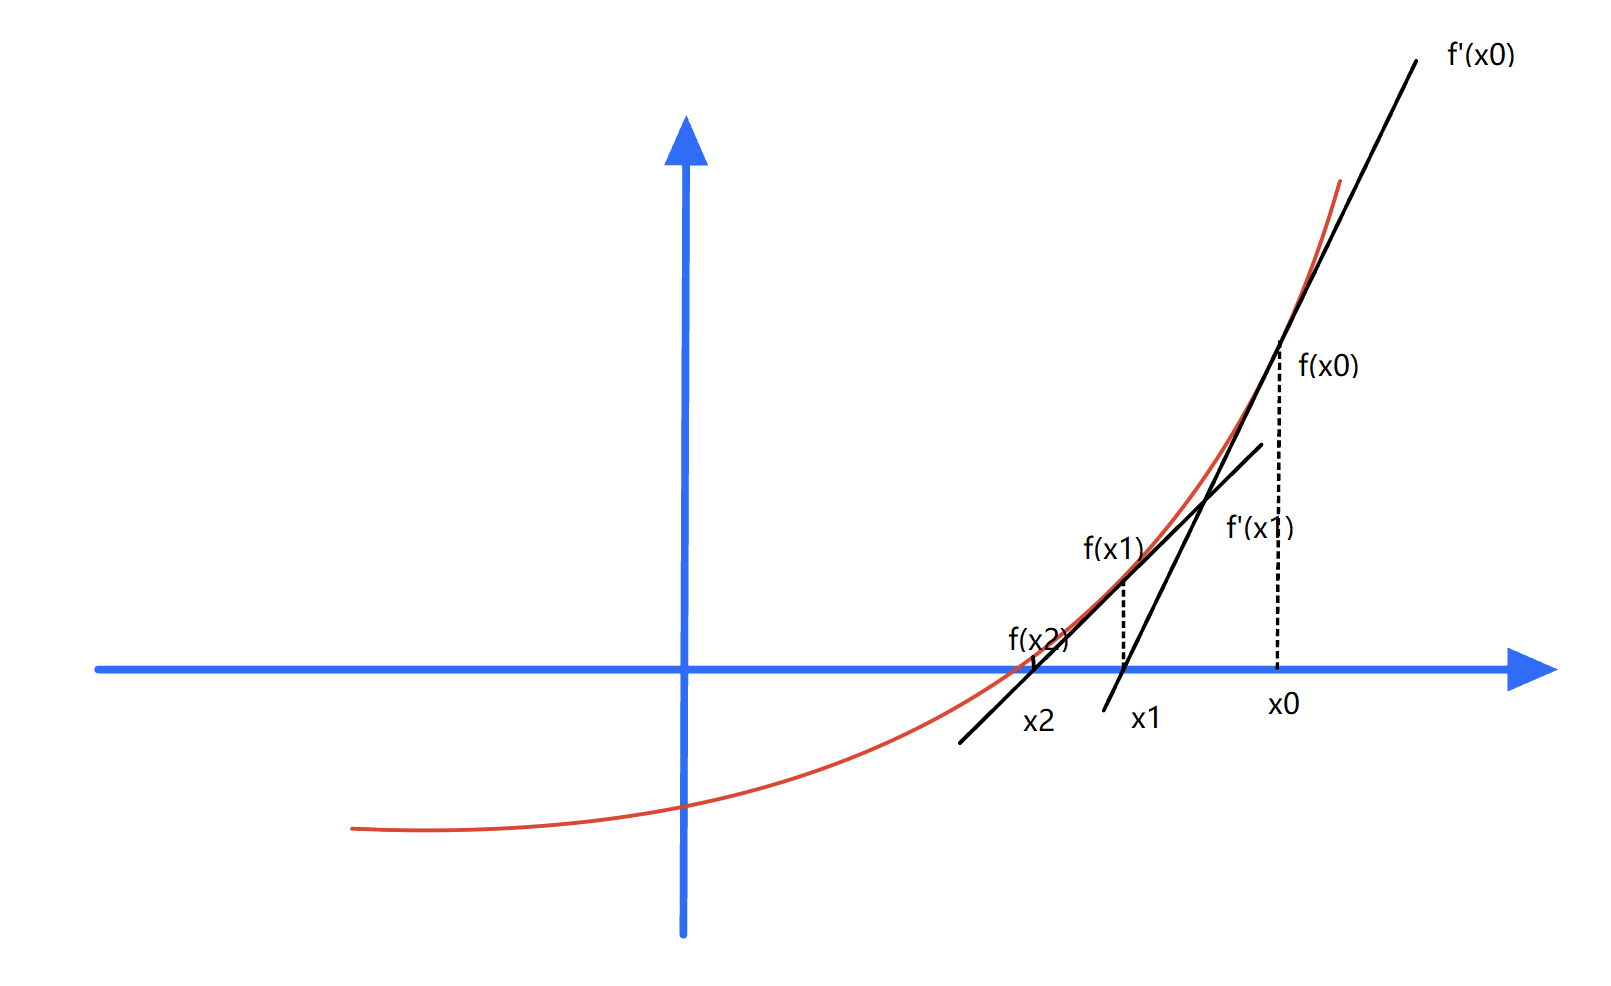
\includegraphics[width=100mm]{./Figures/newton.png}
        \caption{牛顿迭代法过程}
    \end{figure}
    \begin{algorithm}
        \SetKwInOut{Input}{输入}\SetKwInOut{Output}{输出}
        \SetAlgoLined
        \Input{初始点$x_0\in \mathbb{R}^{n},\varepsilon >0,k=0$}
        \Output{最优解$x_{k+1}$}
        \While{未收敛} {
            $d_k=-G_k^{-1}g_k$
            $x_{k+1}=x_k+\alpha_kd_k$
        }
        \caption{牛顿迭代法的算法}
    \end{algorithm}

\subsection{海塞矩阵}
海塞矩阵(Hesse矩阵),是一个多元函数的二阶偏导数构成的方阵,常用于牛顿法解决优化问题:
若一元函数$f(x)$在$x=x_0$点的某个邻域内具有任意阶导数,则$f(x)$在$x_0$点处的泰勒展开式为:
\begin{equation}
    f(x) = f(x_0) + f'(x_0)\Delta x + \frac{1}{2}f''(x_0)(\Delta x)^2 + ..., \Delta x = x - x_0 .
\end{equation}

二元函数$f(x_1,x_2)$在$X_0(x_0,y_0)$点处的泰勒展开式为:
\begin{equation}
    f(x,y) = f(x_0,y_0)
        + \left.\displaystyle\frac{\partial f}{\partial x}\right|_{X_0}\Delta x_0    
        + \left.\displaystyle\frac{\partial f}{\partial y}\right|_{X_0}\Delta y_0    
        + \frac{1}{2}
        \left[ \left.\displaystyle\frac{\partial^2f}{\partial x^2}\right|_{X_0}\Delta x_0^2 + 
            2\left.\displaystyle\frac{\partial^2f}{\partial x\partial y}\right|_{X_0}\Delta x_0\Delta y_0 + 
            \left.\displaystyle\frac{\partial^2f}{\partial y^2}\right|_{X_0}\Delta y_0^2 \right]   
        + ...
\end{equation}
其中$\Delta x = x - x_0$,$\Delta y = y - y_0$.
将上述展开式写成矩阵形式,则有:
\begin{equation}
    f(X) = f(X_0) 
    + \left.( \displaystyle\frac{\partial f}{\partial x},
        \displaystyle\frac{\partial f}{\partial y} )\right|_{X_0}    
        \begin{pmatrix}
                \Delta x \\
                \Delta y
        \end{pmatrix}
    +\newline \frac{1}{2}(\Delta x, \Delta y)
        \left.
        \begin{pmatrix}
            \displaystyle\frac{\partial^2f}{\partial x^2} & \displaystyle\frac{\partial^2f}{\partial x\partial y} \\
            \displaystyle\frac{\partial^2f}{\partial y\partial x} & \displaystyle\frac{\partial^2f}{\partial y^2}
        \end{pmatrix}
        \right|_{X_0}
        \begin{pmatrix}
                \Delta x \\
                \Delta y
        \end{pmatrix} .
\end{equation}
用矩阵表示,则上式可以转化为
\begin{equation}
    f(X) = f(X_0) + \nabla f(X_0)^{\mathbb{T}}\Delta X + \frac{1}{2}X^{\mathbb{T}}G(X_0)\Delta X + ...\quad,
\end{equation}
其中:
\begin{equation}
    G(X_0) = 
        \left.
        \begin{pmatrix}
            \displaystyle\frac{\partial^2f}{\partial x^2} & \displaystyle\frac{\partial^2f}{\partial x\partial y} \\
            \displaystyle\frac{\partial^2f}{\partial y\partial x} & \displaystyle\frac{\partial^2f}{\partial y^2}
        \end{pmatrix}
        \right|_{X_0},
    \Delta X = 
        \begin{pmatrix}
                \Delta x \\
                \Delta y
        \end{pmatrix}.
\end{equation}
$G(X_0)$是$f(x,y)$在$X_0$点处的Hesse矩阵。它是由函$f(x,y)$在$X_0$点处的二阶偏导数所组成的方阵。
将二元函数的泰勒展开式推广到多元函数,则$f(x_1,x_2...,x_n)$在$X_0$点处的泰勒展开式的矩阵形式为:
\begin{equation}
    f(X) = f(X_0) + \nabla f(X_0)^T\Delta X + \frac{1}{2}X^TG(X_0)\Delta X + ...\quad,
\end{equation}
其中:

(1)$\nabla f(X_0) =
    \left.
    \begin{pmatrix}
        \displaystyle\frac{\partial f}{\partial x_1},
        \displaystyle\frac{\partial f}{\partial x_2},
        ...,
        \displaystyle\frac{\partial f}{\partial x_n} 
    \end{pmatrix}\right|_{X_0}^T$,它是$f(X)$在$X_0$点处的梯度。
        
(2)$ G(X_0) = 
        \left.
        \begin{pmatrix}
            \displaystyle\frac{\partial^2f}{\partial x_1^2} & \displaystyle\frac{\partial^2f}{\partial x_1\partial x_2} & \cdots & \displaystyle\frac{\partial^2f}{\partial x_1\partial x_n}\\
            \displaystyle\frac{\partial^2f}{\partial x_2\partial x_1} & \displaystyle\frac{\partial^2f}{\partial x_2^2} & \cdots & \displaystyle\frac{\partial^2f}{\partial x_2\partial x_n}\\
            \vdots & \vdots & \ddots & \vdots\\
            \displaystyle\frac{\partial^2f}{\partial x_n\partial x_1} & \displaystyle\frac{\partial^2f}{\partial x_n\partial x_2} & \cdots & \displaystyle\frac{\partial^2f}{\partial x_n^2}\\
        \end{pmatrix}
        \right|_{X_0}$
        为$f(X)$在$X_0$点处的Hesse矩阵。
\begin{definition}[Hesse矩阵]
    Hesse矩阵是由目标函数 $f(\cdot)$ 在点 $X$ 处的二阶偏导数组成的 $n\times n$ 阶对称矩阵。       
\end{definition}
    
    
\subsection{牛顿迭代法算例}
\begin{example}
    \begin{equation}
        \min f(x)=\frac{3}{2}x^2+\frac{1}{2}y^2-xy-2x,
        x_0 = -2, y_0 = 4.
        \nonumber
    \end{equation}
\end{example}
\begin{solution}
    \begin{equation}
        \nabla f(x,y) = 
        \begin{pmatrix}
            3x-y-2 \\
            -x+y  
        \end{pmatrix},
    \nonumber
    \end{equation}
    由于$g_k=\nabla f(x,y)$,则
    \begin{equation}
    G = \nabla^2f(x,y) = 
        \begin{pmatrix}
            3 & -1\\
            -1 & 1   
        \end{pmatrix}.
    \nonumber
    \end{equation}
    将$x_0=-2,y_0=4$代入$g_k$,得到
    \begin{equation*}    
        g_0=
        \begin{pmatrix}
            -12\\
            6
        \end{pmatrix},
    \end{equation*}
    同时因为$G$为正定矩阵,则存在逆矩阵
    \begin{equation}
        G^{-1} = 
        \begin{pmatrix}
            \frac{1}{2} & \frac{1}{2} \\ 
            \frac{1}{2} & \frac{3}{2}
        \end{pmatrix}.
    \nonumber
    \end{equation}
    将$G^{-1}$代入牛顿迭代公式$x_{k+1} = x_k - G^{-1}g_K$,得到
    \begin{equation}
        x_1 = x_0 - G^{-1}*g_0 = 
        \begin{pmatrix}
            1 \\
            1
        \end{pmatrix}.
    \nonumber
    \end{equation}
    迭代直到满足终止条件。
\end{solution}


\subsection{算法的收敛性及其优缺点}
    基本牛顿方法具有二阶收敛速度,但只有迭代点充分接近$x^*$时,才能保证其收敛性。
    
\begin{theorem}\label{thm2_1}
    设$f(x) \in \mathbb{R}^2, f(x)$的Hesse矩阵$G(x)$满足Lipschitz条件,
    即存在$\beta>0$,对任给的$x$与$y$,有$\|G(x)-G(y)\|\leq\beta\|x-y\|$。
    若$x_0$充分接近$f(x)$的局部极小点$x^*$,且$G^*$正定,
    则牛顿方法对所有的$k$有定义,并以二阶收敛速度收敛。
\end{theorem}
    
    牛顿迭代法的
    \textbf{优点}是:当$x_0$充分接近问题的极小点$x^*$时,方法拥有二阶收敛速度;
    相比于梯度下降法的一阶收敛有着更快的收敛速度。
    由于牛顿法使用二次曲面去拟合当前所处位置的局部曲面,
    而梯度下降法是用一个平面去拟合当前的局部曲面,
    通常情况下,二次曲面的拟合会比平面更好,
    所以牛顿法选择的下降路径会更符合真实的最优下降路径。
    \textbf{缺点}是:当$x_0$没有充分接近问题的极小点$x^*$时,
    $G_k$会出现不正定或奇异的情况,使得${x_k}$不能收敛到$x^*$,甚至无法迭代下去;
    即使$G_k$正定,${f_k}$仍未必单调下降;
    每次使用牛顿法进行计算的时候都需要计算Hesse矩阵,迭代计算量大。
    
    
\subsection{牛顿迭代法的改进}
    为克服牛顿迭代法的缺点,可以通过以下几种方法来改进:
    \subsubsection{阻尼牛顿方法}
        阻尼牛顿法是带一维搜索的牛顿方法。
        牛顿法缺点中,确定了迭代方向之后,迭代步长默认为1,
        但是这个迭代方向并不一定是朝着函数值下降的方向。
        所以阻尼牛顿法为了解决这个问题,
        采取的做法是确定了迭代方向之后,
        还需要在该方向做一维搜索,
        寻找使得在该迭代方向上最优的迭代步长。
        即$x_{k+1}=x_k+\alpha_kd_k$,其中$\alpha_k$是一维搜索的结果。其优点是:对于正定的$G_k$,${f_k}$单调下降;
        即使$x_0$离$x^*$稍远,${x_k}$仍可能收敛到$x^*$。
        对于严格凸函数,采用Wolfe准则的阻尼牛顿法具有全局收敛性,这一点改善了牛顿迭代法的局部收敛性质。
        
    \subsubsection{混合方法}
        为解决牛顿迭代法在迭代过程中可能出现的Hesse矩阵奇异、不正定或牛顿方向与$g_k$几乎正交的情形,
        我们可以采用混合方法。这里我们考虑的方法是将负梯度方法的混合,
        该方法采用牛顿方向,但在Hesse矩阵$G_k$奇异或$d_k$与$g_k$几乎正交时,采用负梯度方向;
        在$G_k$负定,但$G^{-1}_k$存在时,取$d_k=G^{-1}_kg_k$。
        具体算法如下:
        \begin{algorithm}
            \SetKwInOut{Input}{输入}\SetKwInOut{Output}{输出}
            \SetAlgoLined
            \Input{初始点$x_0\in \mathbb{R}^{n},\varepsilon>0,k=0$}
            \Output{最优解$x_{k+1}$}
            \While{未收敛} {
                \If{$G_k$非奇异}{
                    由牛顿方程求得$d_k$  
                    \If{$g^T_kd_k>\varepsilon_1\|g_k\|\|d_k\|$}{
                        $d_k=-d_k$
                    }
                    \ElseIf{$|g_k^Td_k|\leq\varepsilon_1\|g_k\|\|d_k\|$}{
                        $d_k=-g_k$
                    }
                }
                \Else{
                    $d_k=-g_k$
                }
                线搜索求$\alpha_k,x_{k+1}=x_k+\alpha_kd_k,k=k+1$
            }
            \caption{混合算法的算法}
        \end{algorithm}
            
    \section{拟牛顿方法}
        牛顿迭代法的缺点是每部都需要计算Hesse矩阵$G_x$,
        $G_x$可能奇异或不正定,所以构造了拟牛顿法,既不需要计算二阶偏导数,同时又有较快的收敛速度。
        拟牛顿迭代法的基本思想是利用$x_k$,$x_{k+1}$及其一阶信息构造一个正定的矩阵$B_{k+1}\approx G_{k+1}$,
        此时产生的下降方向$d_{k+1}$满足:$B_{k+1}d_{k+1}=-g_{k+1}$。
        利用上述同样的信息构造一个正定的矩阵$H_{k+1}\approx G_{k+1}^{-1}$此时产生的下降方向$d_{k+1}$
        满足:$d=-H_{k+1}g_{k+1}$。
        
        其中$B_{k+1}\approx G_{k+1}$,满足如下拟牛顿方程:$B_{k+1}s_k=y_k$。
        
        若记$H_{k+1}=B_{k+1}^{-1}$,则$H_{k+1}$应满足$H_{k+1}y_k=s_k$。
        
        下面以矩阵$H_k$为例,给出一般拟牛顿法的结构。             
        \begin{algorithm}
            \SetKwInOut{Input}{输入}\SetKwInOut{Output}{输出}
            \SetAlgoLined
            \Input{初始点$x_0\in \mathbb{R}^{n}$,对称正定阵$H_0\in \mathbb{R}^{n\times n},\varepsilon >0,k=0$}
            \Output{最优解$x_{k+1}$}

            \While{未收敛} {
                $d_k=-H_kg_k$
                
                沿方向$d_k$进行线搜索求$\alpha_k>0$,$x_{k+1}=x_k+\alpha_kd_k$
                
                修正$H_k$得$H_{k+1}$,使$H_{k+1}$满足$H_{k+1}y_k=s_k,k=k+1$
            }
            
            注:$H_k$的选取和修正是关键,
            通常$H_0=I$,则$d_0=-g_0;H_{k+1}=H_k+\Delta H_k$。
            \caption{拟牛顿方法的算法}
        \end{algorithm}
        
\subsection{各种拟牛顿方法及其优缺点}
\subsubsection{SR1}
    SR1方法\cite{1980Curvilinear}也即对对称秩1方法更新,根据$x_k$处的信息得到一个修正量$\Delta H_k$
    来直接加上$H_k$来更新,也就是如下的式子:
    \begin{equation}
        H_{k+1} = H_k + \Delta H_k,
        \nonumber
    \end{equation}
    由于我们希望$\Delta H_{k+1} \approx \nabla^2f(x_{k+1})^{-1},
                    \Delta H_{k} \approx \nabla^2f(x_k)^{-1}$,
    所以有$\Delta H_k \approx \nabla^2f(x_{k+1})^{-1}-\nabla^2f(x_k)^{-1}$。

    由于$\nabla^2f(x_{k+1})^{-1}$和$\nabla^2f(x_k)^{-1}$都是对称矩阵,
    所以$\Delta H_k$也是对称矩阵。
    SR1算法将$\Delta H_k$设为$\beta uu^T$,则迭代式为:
    \begin{equation}
        H_{k+1} = H_{k} + \beta uu^T, \beta\in \mathbb{R}, u \in \mathbb{R}^{n}.
    \nonumber
    \end{equation}
    
    \textbf{优点:}
        SR1算法可以使得最终选择的$B_k$会一步步的接近于函数的Hesse矩阵,
        它之后会越来越逼近Hesse矩阵,可以恢复牛顿法的二次局部收敛速度。
        不需要一维搜索,而具有二次终止性;
        具有遗传性:$H_iy_j=s_j,j<i.$。
    
    \textbf{缺点:}
        矩阵$B_k$不保正定,如果使用线搜索会导致无法找到下降方向的问题,
        使得SR1校正不保持迭代矩阵$H_k$的正定性,
        仅当$(s_k-H_ky_k)^Ty_k>0$时,
        SR1校正才具有正定性。
        另一方面,矩阵可以很好的逼近Hesse矩阵,
        但是线搜索每一次只会利用到一个方向上的Hesse矩阵的信息。
        
\subsubsection{DFP}
    DFP方法\cite{1963A}是在SR1的方法基础上对于$\Delta H$进行进一步更新,
    相对于SR1令$\Delta H_k = \beta uu^T$,
    DFP提供了更大的自由度,令$\Delta H_k = \beta uu^T + \gamma vv^T$,
    则此时$H_k$的迭代更新式为:
    \begin{equation}
        H_{k+1} = H_{k} + \beta uu^T + \gamma vv^T.
        \nonumber
    \end{equation}
    
    \textbf{优点:}
        DFP法只需计算一阶偏导数,
        无需计算二阶偏导数及其逆矩阵,
        对于二次函数具有二次终止性;
        对目标函式的初始点选择均无严格要求,收敛速度快;
        为提高实际计算的稳定性,除提高一维搜寻的精度外,
        通常还将进行$n$次迭代作为一个循环,
        并以上一循环的终点作为起点继续进行循环叠代,
        使得其对于一般函数校正保持正定性;
        当采用精确线搜索时,对于凸函数具有总体收敛性。
    
    \textbf{缺点:}
        DFP方法具有数值不稳定,有时产生数值上的Hesse近似。
        
\subsubsection{BFGS}
    BFGS方法\cite{1989On}在DFP方法的基础上,对于$\nabla^2f(x_k)$进行近似,令$B_k=\nabla^2f(x_k)$,得到
    \begin{equation}
        B_{k+1} = B_k + \beta uu^T + \gamma vv^T.
        \nonumber
    \end{equation}
    
    \textbf{优点:}
        具有DFP校正所有的各种性质,同时克服了DFP方法的上述缺点;
        当采用Goldstein或Wolfe线搜索时,
        BFGS公式还具有总体收敛性;
        数值执行中,BFGS公式也优于DFP公式,
        尤其是它常常能与低精度线搜索方法一起使用。
    
\subsection{算例分析}
\begin{example}\label{nndfl}
    考虑问题
    \begin{equation}
        \min f(x) = \sum^m_{i=1}r_i^2(x), n=6,m\geq n,
        \nonumber
    \end{equation}
        其中,
        $r_i(x)=x_3e^{-t_ix_1}-x_4e^{-t_ix_2}+x_6e^{-t_ix_5}-y_i$,
        $t_i=0.1i$,
        $y_i=e^{-t_i}-5e^{-10t_i}+3e^{-4t_i}$.
    
    \begin{table}[htbp]\center
        \caption{$\sigma = 0.1$时,SR1,BFGS与DFP三种方法的
                \\迭代次数和函数调用次数}
        \begin{tabular}{cccccccccccc}
        \toprule %添加表格头部粗线
            \multicolumn{3}{c}{m}& 
            \multicolumn{2}{c}{SR1}&&                  \multicolumn{2}{c}{BFGS}&&                 \multicolumn{2}{c}{DFP}&\\
        \cmidrule(lr){4-12}
            \multicolumn{2}{c}{}&&ite&feva&&ite&feva&&ite&feva&\\  %有n个&,就表示该行有n+1列
        \hline %绘制一条水平横线
            \multicolumn{2}{c}{6} & &113&746 & &14&102& &314&1935& \\
            \multicolumn{2}{c}{7} & &52 &481 & &49&303& &18 &128 & \\
            \multicolumn{2}{c}{8} & &172&1251& &27&126& &182&874 & \\
            \multicolumn{2}{c}{9} & &17 &111 & &27&137& &197&1233& \\
            \multicolumn{2}{c}{10}& &11 &68  & &88&460& &128&686 & \\
            \multicolumn{2}{c}{11}& &28 &186 & &25&110& &187&959 & \\
            \multicolumn{2}{c}{12}& &22 &130 & &24&98 & &9  &71  & \\
            \multicolumn{2}{c}{13}& &16 &119 & &28&124& &24 &112 & \\
        \bottomrule %添加表格底部粗线
        \end{tabular}
        \label{nndf1}
    \end{table}
    
    \begin{table}[htbp]\center
        \caption{$\sigma = 0.1$时,SR1,BFGS与DFP三种方法的
                \\所得解点$x_k$处的$\|g_k\|_\infty$}
        \begin{tabular}{ccccccccccc}
        \toprule %添加表格头部粗线
            \multicolumn{2}{c}{m}&& 
            \multicolumn{2}{c}{SR1}&                   \multicolumn{2}{c}{BFGS}&                  \multicolumn{2}{c}{DFP}&\\
        \hline %绘制一条水平横线
            \multicolumn{2}{c}{6} & &7.05e-5& &2.74e-0& &1.20e-1& \\
            \multicolumn{2}{c}{7} & &4.54e-6& &1.09e-4& &3.85e-1& \\
            \multicolumn{2}{c}{8} & &6.23e-5& &1.04e-6& &1.54e-1& \\
            \multicolumn{2}{c}{9} & &7.59e-9& &1.81e-5& &6.35e-1& \\
            \multicolumn{2}{c}{10}& &9.71e-6& &2.14e-5& &9.44e-1& \\
            \multicolumn{2}{c}{11}& &4.57e-3& &2.04e-6& &6.93e-3& \\
            \multicolumn{2}{c}{12}& &5.87e-4& &8.40e-2& &1.14e-1& \\
            \multicolumn{2}{c}{13}& &2.50e-1& &4.13e-7& &6.14e-6& \\
        \bottomrule %添加表格底部粗线
        \end{tabular}
        \label{nndf2}
    \end{table}
\end{example}

对例\ref{nndfl}而言,DFP的方法的有效性明显低于BFGS方法。
在表\ref{nndf1}中,ite表示迭代次数,feva表示调用函数的次数
可以看到DFP方法大部分情况下的迭代次数都超过BFGS方法,
而调用次数DFP方法多数情况下也多于BFGS方法。
而SR1方法所需的函数调用次数和所得结果的精确度与BFGS方法更相近,
但SR1方法不如BFGS方法稳定。

实际上,DFP方法对于许多问题都有类似的数值表现。
在表\ref{nndf2}中,DFP的解梯度值远超过SR1和BFGS的方法
同时注意到,BFGS方法在m=6,12时,解点的梯度值$\|g_k\|_\infty$不小,
这是由于在$k-1$步迭代,找到的$x_k$不能使函数值有足够的下降,从而导致
$f_{k+1}-f_{k}$满足精度要求,停止迭代造成的。
